
\documentclass[calculator,steamtables,refrigeranttables,psychrometricchart,datasheet,solutions]{exam}
%\documentclass[calculator,steamtables,refrigeranttables,psychrometricchart,datasheet]{exam}

% The full list of class options are
% calculator : Allows approved calculator use.
% datasheet : Adds a note that data sheet are attached to the exam.
% handbook : Allows the use of the engineering handbook.
% resit : Adds the resit markings to the paper.
% sample : Adds conspicuous SAMPLE markings to the paper
% solutions : Uses the contents of \solution commands (and \solmarks) to generate a solution file

\usepackage{pdfpages} 
\usepackage{lscape,comment}

\coursecode{EG501J}%%
\coursetitle{Renewable Energy: Solar and Geothermal}%
%\coursecode{EG3539}%
%\coursetitle{Thermodynamics}%

\examtime{00.00--00.00}%
\examdate{00}{12}{2014}%
\examformat{Candidates must attempt \textit{all} questions.}

\newcommand{\frc}{\displaystyle\frac}
\newcommand{\br}[1]{\!\left( #1 \right)}
\newcommand{\abs}[1]{\left| #1 \right|}
\newcommand{\fracd}[2]{\frac{\mathrm{d} #1}{\mathrm{d} #2}}
\newcommand{\fracp}[2]{\frac{\partial #1}{\partial #2}}
\renewcommand{\d}[1]{\mathrm{d} #1 } 
\newcommand{\Ma}{\mathrm{M\!a}} 



\begin{document}

%%%
%%% Question 01 
%%%
\begin{question} %\vspace{-2\baselineskip} 
A binary geothermal power station is operated with brine extracted at 90$^{\circ}$C and reinjected at 30$^{\circ}$C. Propane $\left(\text{n-C}_{3}\right)$ is used as working fluid in the Rankine cycle to produce power $\left(W_{T}\right)$ in a turbine (isentropic expansion) with efficiency $\left(\eta_{T}\right)$ of 90$\%$.  After condensated, n-C$_{3}$ is driven to a heat exchanger (with thermal efficiency of 68$\%$) and the cycle continues. The mass flow rate of n-C$_{3}$ $\left(\dot{m}_{C3}\right)$ is 250 kg.s$^{-1}$ and the heat capacity $\left(C_{p}\right)$ of brine is 3565.5 J.(kg.K)$^{-1}$. Conditions for n-C$_{3}$ and brine flows are described in Table~\ref{exam1_table1}.

\begin{figure}[h]
\begin{center}
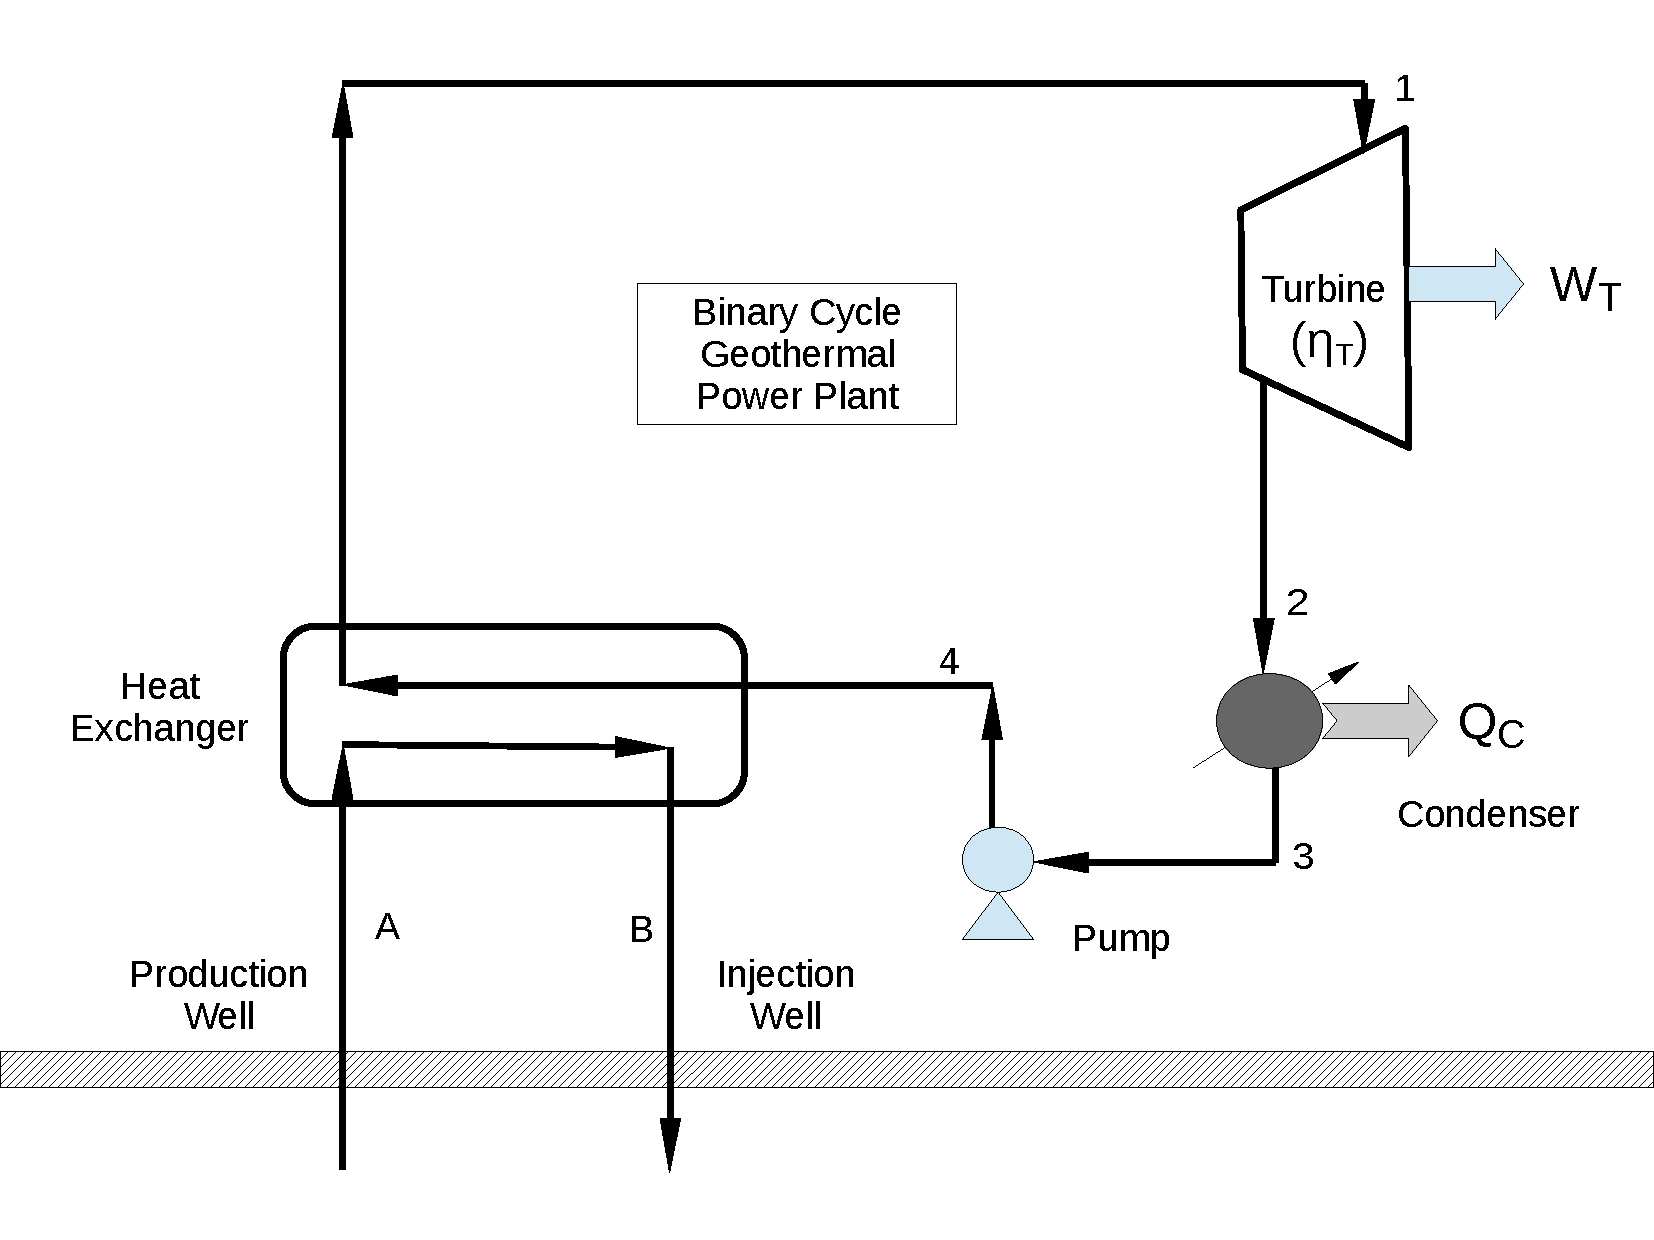
\includegraphics[width=8.cm,height=6.cm,clip]{./Pics/GeothermalBinaryCycle}
%\caption{ Reheat and regenerative Rankine cycle with 2 turbines.}
\label{exam_mod02_rankinecycle}
\end{center}
\end{figure}\vspace{-1cm}
\begin{table}[!h]
\caption{Thermodynamic table of the geothermal binary cycle.}% (Question 1).}
\begin{center}
\begin{tabular} {||c | c c c c c || }
\hline\hline
{\bf Stage} & {\bf P}    & {\bf T}        & {\bf State}    & {\bf H}             & {\bf S}                  \\
            & {\bf (bar)}& {\bf ($^{o}$C)} &               & {\bf (kJ.kg$^{-1}$)} & {\bf (kJ.(kg.K)$^{-1}$)}  \\
\hline\hline
 {\bf 1 }   & 16         & 50             &   {\bf (a)}    & {\bf (b)}           & {\bf (c)}                \\
 {\bf 2 }   & 6          &  --            &   wet vapour   & {\bf (d)}           & --                       \\
 {\bf 3 }   & 6          &                &   sat. liquid  & {\bf (e)}           & --                       \\
 {\bf 4 }   & 16         &                &   {\bf (f)}    & {\bf (g)}           & --                       \\
 {\bf A }   & --         & 90             &   --           & --                  & --                       \\
 {\bf B }   & --         & 30             &   --           & --                  & --                       \\
 \hline\hline
\end{tabular}
\end{center}
\label{exam1_table1}
\end{table}

\begin{enumerate}[(a)]
%%
%% Question 1
%%
\item In Table \ref{exam1_table1}, determine {\it (a)-(g)}.~\marks{7}%{\bf [10 Marks]}
%
\solution{
In order to fill the Table we need to calculate the thermodynamic properties for each stage of the cycle:
\begin{description}
%%%
\item[Stage 1:] At P$_{1}$ = 16 bar, T$_{1}$ = 50$^{\circ}$C $>$ T$_{sat}\left(P_{1}\right)$ = 46.89$^{\circ}$C. Therefore the fluid is at {\bf superheated state}~\solmarks{1/7}. From the superheated table for n-C$_{3}$ at P$_{1}$ and T$_{1}$, we can obtain:\\
{\bf H$_{1}$ = 522.5 kJ.kg$^{-1}$}~\solmarks{1/7} and\\
{\bf S$_{1}$ = 1.733 kJ.(kg.K)$^{-1}$}~\solmarks{1/7}. 
%%%
\item[Stage 2:] At P$_{2}$ = 6 bar, the fluid is wet vapour after the isentropic expansion. We should first calculate the quality of the vapour in an ideal expansion (using values of entropy/enthapy obtained from the saturated n-C$_{3}$ table at P$_{2}$.
\begin{displaymath}
x_{2s} =\frc{S_{2s}-S_{f}}{S_{g}-S_{f}} = \frc{1.733 - 0.446}{1.737-0.446} = 0.9969
\end{displaymath}
now to calculate the ideal enthalpy,
\begin{displaymath}
x_{2s} = 0.9969 = \frc{H_{2s}-H_{f}}{H_{g}-H_{f}} = \frc{H_{2s}-115.3}{478.3-115.3}\;\;\Longleftrightarrow\;\; H_{2s} = 477.17 \frc{kJ}{kg}
\end{displaymath}
As the efficiency of the turbine is of 90$\%$,
\begin{displaymath}
\eta_{\text{Turbine}} = 0.90 =\frc{H_{2}-H_{1}}{H_{2s}-H_{1}} = \frc{H_{2} - 522.5}{477.17 - 522.5} \;\;\Longleftrightarrow \;\; {\bf H_{2} = 481.70\frc{kJ}{kg}}
\end{displaymath}~\solmarks{1/7}
%%%
\item[Stage 3:] At P$_{3}$ = P$_{2}$ = 6 bar, the fluid leaving the condenser towards the pump is saturated liquid, and the enthalpy and specific volume are the same of the liquid phase obtained fromthe saturated table:\\
{\bf H$_{3}$} = H$_{f}\left(\text{P = 6 bar}\right)$ {\bf = 115.3 kJ.kg$^{-1}$}~\solmarks{1/7} \\
V$_{3}$ = V$_{f}\left(\text{P = 6 bar}\right)$ = 1.931$\times$10$^{-3}$ m$^{3}$.kg$^{-1}$ 
%%%
\item[Stage 4:] The fluid leaving the pump is {\bf sub-cooled liquid}~\solmarks{1/7}. As there is no heat loss in the pump, we can assume $dH \approx VdP$, therefore
\begin{displaymath}
{\bf H_{4}} = H_{3} + V_{3}\left(P_{4}-P_{3}\right) = 115.3\frc{kJ}{kg} + 1.931\times 10^{-3} \frc{m^{3}}{kg} \left(16 - 6\right)\text{bar} {\bf= 117.23 \frc{kJ}{kg}}
\end{displaymath}~\solmarks{1/7}

\end{description}
Thus the Table becomes:
\begin{center}
\begin{tabular} {||c | c c c c c || }
\hline\hline
{\bf Stage} & {\bf P}    & {\bf T}        & {\bf State}    & {\bf H}             & {\bf S}                  \\
            & {\bf (bar)}& {\bf ($^{o}$C)} &               & {\bf (kJ.kg$^{-1}$)} & {\bf (kJ.(kg.K)$^{-1}$)}  \\
\hline\hline
 {\bf 1 }   & 16         & 50             &{\bf superheated vapour}&{\bf 522.5}  & {\bf 1.733}              \\
 {\bf 2 }   & 6          &  --            &   wet vapour   & {\bf 481.70}        & --                       \\
 {\bf 3 }   & 6          &                &   sat. liquid  & {\bf 115.3}         & --                       \\
 {\bf 4 }   & 16         &                &{\bf sub-cooled liquid}& {\bf 117.23} & --                       \\
 {\bf A }   & --         & 90             &   --           & --                  & --                       \\
 {\bf B }   & --         & 30             &   --           & --                  & --                       \\
 \hline\hline
\end{tabular}
\end{center}
}
%%
%% Question 2
%%
\item Calculate the power produced by the turbine $\left(W_{T}\right)$ in {\it MW}.~\marks{1}
%
\solution{
\begin{displaymath}
{\bf W_{T}} = \dot{m}_{C3} \left(H_{1}-H_{2}\right) = 250\frc{kg}{s} \times \left(522.5 - 481.70\right)\frc{kJ}{kg} = 10200 \frc{kJ}{s} {\bf = 10.2 MW}
\end{displaymath}~\solmarks{1/1}
}
%%
%% Question 3
%%
\item Assuming that the heat exchanger has an efficiency of 68$\%$, calculate the mass flow rate of brine in {\it kg.s}$^{-1}$.~\marks{3}
%
\solution{
The heat extracted by the n-C$_{3}$ $\left(\dot{Q}_{C3}\right)$ fluid in the heat exchanger can be easily calculated by
\begin{displaymath}
{\bf \dot{Q}_{C3}} = \dot{m}_{C3}\left(H_{1}-H_{4}\right) {\bf = 101317.5\frc{kJ}{s}}
\end{displaymath}~\solmarks{1/3}
Assuming that the heat extracted from the geothermal fluid (brine), $\dot{Q}_{gf}$ is transferred to the n-C$_{3}$ stream with efficiency of 68$\%$,
\begin{displaymath}
\eta_{\text{HE}} = 0.68 = \frc{\dot{Q}_{C3}}{\dot{Q_{gf}}} \;\; \Longleftrightarrow  {\bf \dot{Q}_{gf} = 148996.32 \frc{kJ}{s}}
\end{displaymath}~\solmarks{1/3}
With the heat generated by the geothermal fluid and the inlet/outlet fluid temperatures, we can now calculate the brine mass flow rate for the associated heat transferred,
\begin{displaymath} 
\dot{Q}_{gf} = 148996.32 \frc{kJ}{s} = \dot{m}_{gf} C_{p} \left(T_{A} - T_{B}\right)  \;\;\Longleftrightarrow\;\; {\bf \dot{m}_{gf} = 696.57\frc{kg}{s}}
\end{displaymath}~\solmarks{1/3}
}
%%%
%%% Question 4
%%%
\item Sketch the temperature $\times$ entropy (TS) diagram for the process indicating the liquid and vapour saturated lines and each stage of the n-C$_{3}$ Rankine cycle.~\marks{4}
%
\solution{
\begin{center}
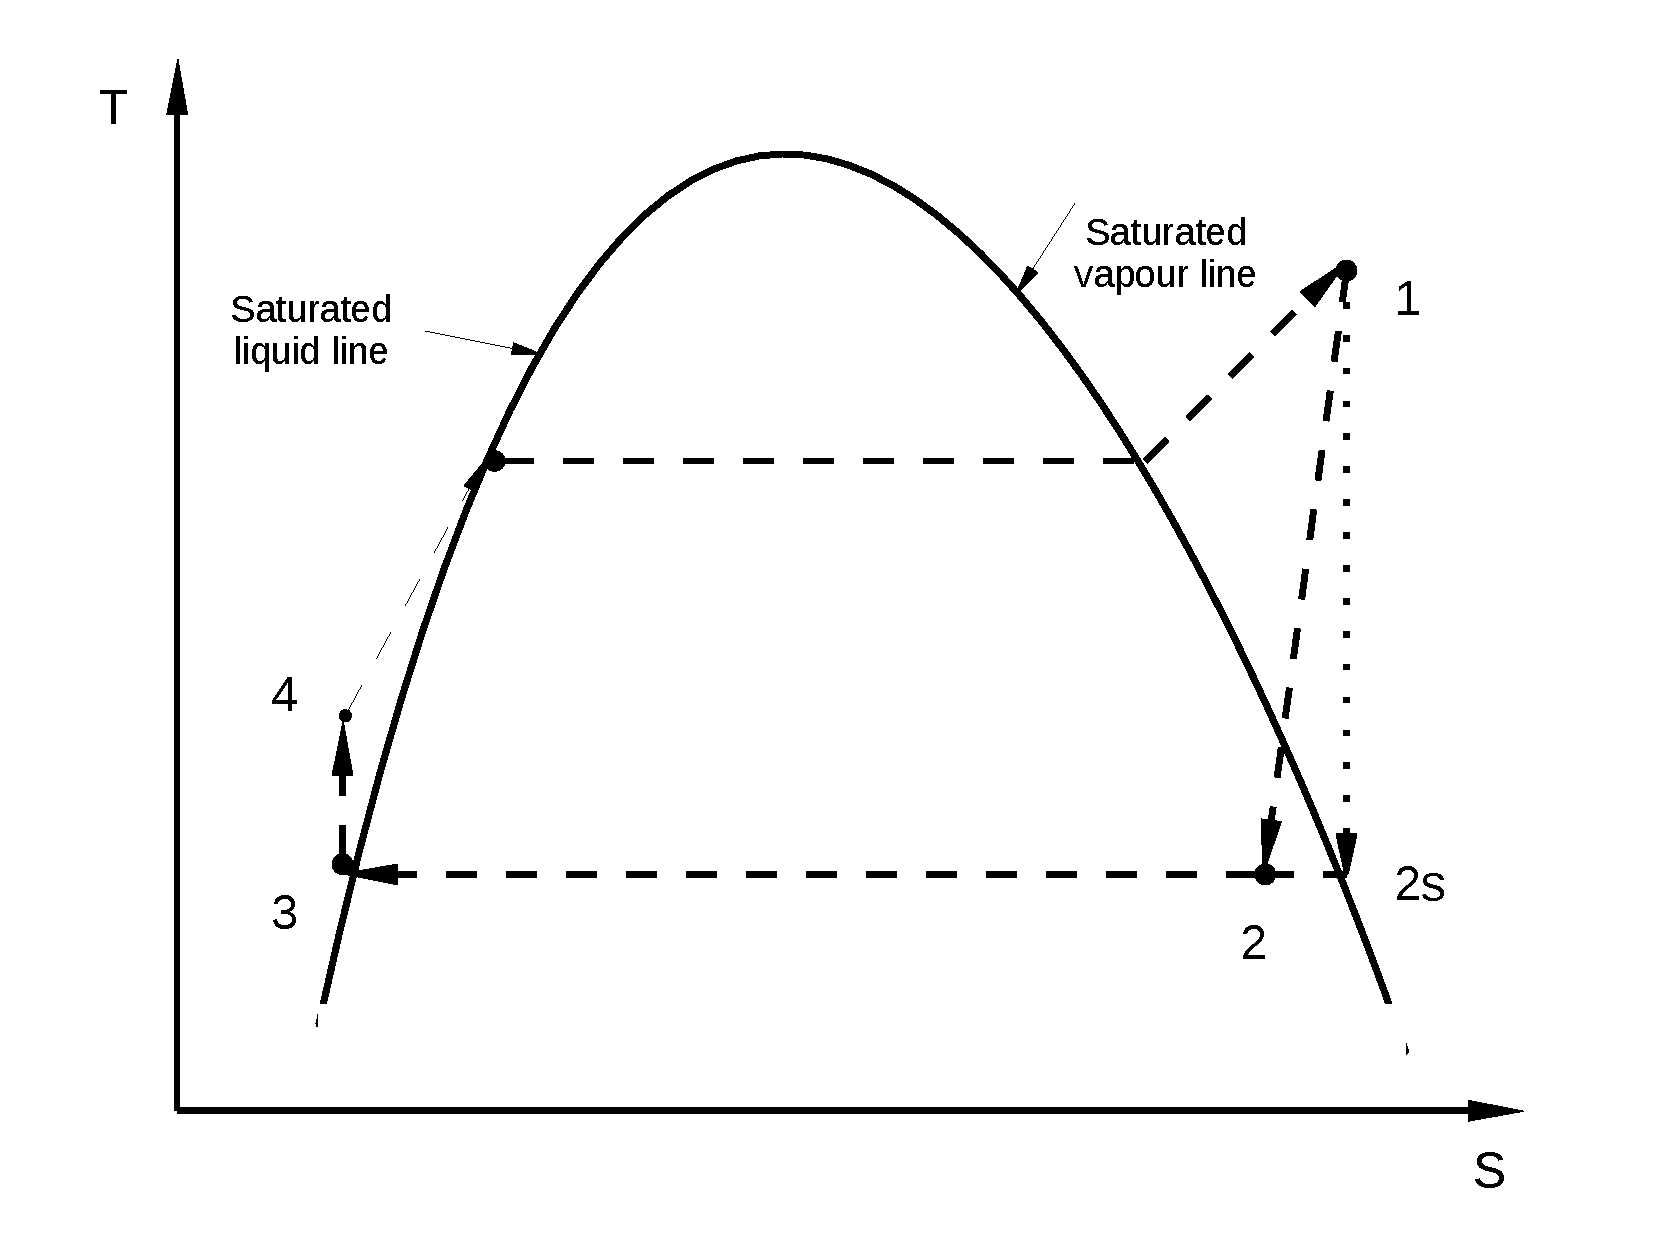
\includegraphics[width=8.cm,clip]{./Pics/TS_DIagramGeothermalBinary}
\end{center}~\solmarks{5/5}
}
%%%
%%% Question 4
%%%
\item Dry-steam, flash-steam and binary-cycle power plants are considerend the three main conversion technologies in geothermal systems. Describe the flash-steam process.~\marks{4} 
%
\solution{
\begin{enumerate}
\item It is the most common geothermal power plant system and usually operates at temperatures above 150$^{\circ}$C;~\solmarks{0.5/4}
\item It utilises water below the boiling point at reservoir conditiions that suffer an isenthalpic flash at lower surface pressures;~\solmarks{1/4}
\item During the flash, steam is driven to a turbine to undertae an isentropic expansion producing work (i.e., power);~\solmarks{1/4}
\item After moving the turbine, the steam is condensed and reinjected;~\solmarks{1/4}
\item The liquid fluid produced during the flash is chemically treated and re-injected into the well.~\solmarks{0.5/4}
\end{enumerate}
}

%%%
%%% Question 5
%%%
\item  Temperature gradient $\left(\nabla T\right)$ between upper and deep layers of rocks (i.e., near the surface and at large depths) can lead to geothermal circulation. Define thermal buoyancy and its links to thermal convection.~\marks{6}
%
\solution{
Let's consider a geothermal reservoir with dimension $\underline{X} \left(=x, y, z\right)$ with {\bf imposed temperature gradient $\left(\nabla T = \frac{\partial T}{\partial z}\right)$}~\solmarks{1/6} and saturated with fluid with density 
\begin{displaymath}
\rho=\rho\left(T, p, \underline{X}, \text{salinity, etc}\right).
\end{displaymath} 
Under static conditions, pressure can be expressed as {\bf $p = \rho g z$}~\solmarks{1/6}. Algebraic expressions, known as {\bf equations of state (EOS), are designed to correlate density, temperature, pressure and any other thermodynamic potential}~\solmarks{1/6}. The pressure can be obtained by integrating the above equation through the depth,
\begin{displaymath}
p(z) = \int\limits_{0}^{z}\rho(z) g dz
\end{displaymath} 
{\bf Thermal buoyancy is a physical phenomena in which cold and denser fluid at low depth $\left(z\rightarrow 0\right)$ displaces warm and lighter fluid at larger depth pushing the warmer fluid upwards.}~\solmarks{3/6} 
} 

 
 
%
\end{enumerate}

To solve this problem, you should assume that the saturated liquid streams are incompressible, and therefore $dH = VdP$ (where $H$, $V$ and $P$ are enthalpy, volume and pressure, respectively). Quality of the vapour is expressed as
\begin{displaymath}
x_{j} = \frc{\Psi_{j}-\Psi_{f}}{\Psi_{g}-\Psi_{f}}\;\;\;\text{with }\Psi=\left\{H,S\right\}
\end{displaymath}
where $S$ is the entropy. Efficiency of the turbine $\left(\eta_{\text{Turbine}}\right)$ and the heat exchanger $\left(\eta_{\text{HE}}\right)$ are given by,
\begin{displaymath}
\eta_{\text{Turbine}} =\frc{H_{2}-H_{1}}{H_{2s}-H_{1}} \;\;\;\text{ and }\;\;\; \eta_{\text{HE}} = \frc{\dot{Q}_{C3}}{\dot{Q_{gf}}}
\end{displaymath}
where $H_{2s}$ is the enthalpy of stream $2$ assuming ideal turbine performance (i.e., reversible expansion). $\dot{Q}_{C3}$ and $\dot{Q}_{gf}$ are the heat associated with the n-C$_{3}$ and brine streams, respectively, at the heat exchanger.

\end{question}

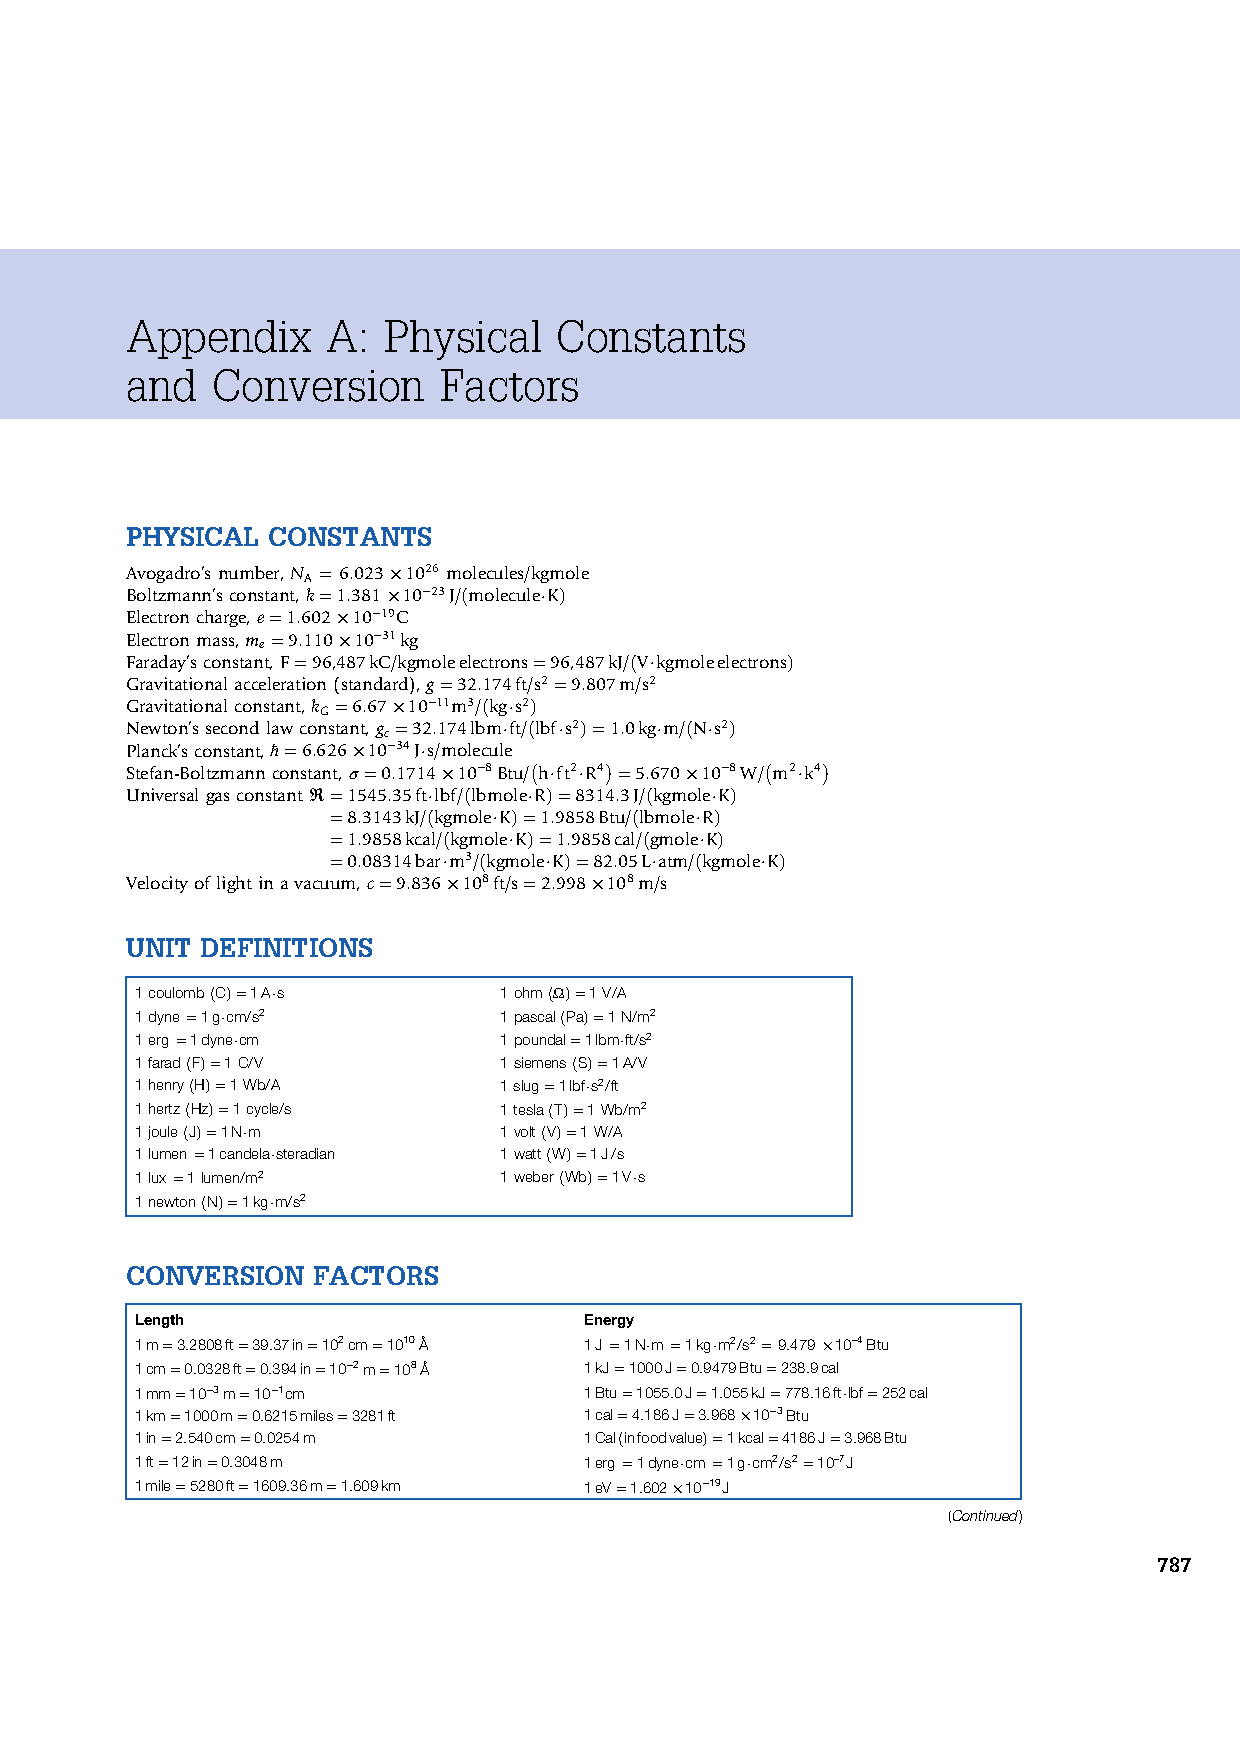
\includepdf[pages={1-6}]{./Pics/nC3_UnitConv}

\clearpage
\end{document}
